\chapter{Pygame Invaders: Η Εισβολή Αρχίζει!}
\label{chap:pygame-invaders-invasion}
\section{Εισαγωγή}
Καθώς φαίνεται τα ψέματα τελείωσαν. Έχουμε το σκάφος μας, το κινούμενο φόντο, το Laser και στο προηγούμενο κεφάλαιο μας ήρθαν μια\ldots{} βόλτα και οι πρώτοι εξωγήινοι.  Λίγο διστακτικοί εμείς, τους κοιτάξαμε, τους ρίξαμε και διαπιστώσαμε ότι δεν γίνεται τίποτα! Μα τι λείπει επιτέλους από αυτό το παιχνίδι;

Αν είχατε ξεκινήσει το programming παιχνιδιών πριν μερικά χρόνια --- τότε που η δημιουργία frame based shooters ήταν απλώς άπιαστο όνειρο --- και περιγράφατε το πρόβλημα σας στο φίλο σας που έγραφε εκείνη την εποχή το δικό του Invaders θα σας έλεγε δύο λέξεις: \emph{collision detection}. Η \emph{ανίχνευση συγκρούσεων} είναι ένα βασικό θέμα (και πρόβλημα) σε όλα τα παιχνίδια δράσης. Είναι το τμήμα του προγράμματος που αναγνωρίζει πότε ο εξωγήινος δέχτηκε τη βολή, πότε το διαστημόπλοιο έσκασε πάνω στον\ldots{} κακόβουλα κινούμενο μετεωρίτη, πότε ο pacman έφαγε το φαντασματάκι.

Μια κακοσχεδιασμένη ρουτίνα ανίχνευσης συγκρούσεων οδηγεί σε τραγελαφικά αποτελέσματα:
%
\begin{itemize}
\item[-] Χαρακτήρες που περνάνε μέσα από\ldots{} τοίχους (μόνο ο κώδικας μας και τα φαντάσματα το καταφέρνουν αυτό)
\item[-] Βολές που ακουμπάνε --- ή ακόμα χειρότερα περνάνε μέσα --- από χαρακτήρες χωρίς να τους καταστρέφουν. Και καλά να είναι το δικό μας διαστημόπλοιο, τι γίνεται με τυχόν\ldots{} απέθαντους εξωγήινους;
\item[-] Laser που καταστρέφουν πράγματα τα οποία δεν φαίνονται να έχουν αγγίξει ή --- ακόμα χειρότερα --- βρίσκονται στην\ldots{} άλλη άκρη της οθόνης.
\end{itemize}

Σε ένα παιχνίδι που δεν έχει γραφτεί με τη frame based λογική που χρησιμοποιούμε εδώ, η ανίχνευση συγκρούσεων δεν είναι και το πιο εύκολο πράγμα: φανταστείτε ότι αν η γλώσσα  παρέχει αυτόνομα κινούμενα sprites, το πρόγραμμα μας μπορεί να εκτελεί οποιαδήποτε τυχαία εντολή την ώρα που θα συγκρουστούν. Αν είμαστε τυχεροί, η εντολή που θα εκτελείται θα είναι αυτή που θα εντοπίζει τη σύγκρουση δύο sprites.

Για να αντιμετωπιστεί το πρόβλημα αυτό, σε κάποιες διαλέκτους BASIC της εποχής άρχισαν να εμφανίζονται εντολές με λογική events (συμβάντων): το πρόγραμμα εκτελούνταν κανονικά, η γλώσσα έλεγχε αυτόματα κατά τακτά διαστήματα για συγκρούσεις και έστελνε ένα event στο πρόγραμμα το οποίο μετά επεξεργαζόμασταν  για να δούμε τι\ldots{} σκοτώθηκε.  Αυτά για τους λίγους τυχερούς βέβαια  με τους αντίστοιχους υπολογιστές -- εμείς ήμασταν καταδικασμένοι να πυροβολάμε δέκα φορές το κάθε καταραμένο UFO μέχρι να εκτελεστεί η σωστή εντολή!

Και τώρα που έχουμε frames τι γίνεται; Τα πράγματα έχουν απλοποιηθεί πολύ! Πάμε να τα δούμε.
%
\section{Collision Detection, Part I -- Εξωγήινε σε Έφαγα!}
%
Ρίξτε λίγο μια ματιά στο super class {\tt Craft} και θα θυμηθείτε ότι έχουμε αποθηκεύσει τις συντεταγμένες του σκάφους (είτε του δικού μας είτε του εξωγήινου) σε ένα αντικείμενο τύπου {\tt Rect}:

\begin{minted}[bgcolor=bg, frame=lines, framesep=10pt]{python}
    self.rect = pygame.Rect(coord,(self.ship_width, self.ship_height))
\end{minted}

Το παραπάνω μας έχει ήδη διευκολύνει στην κίνηση, καθώς μπορούμε με ένα αντικείμενο rect να αλλάξουμε τις συντεταγμένες επιτόπου, όπως φαίνεται στην ρουτίνα κίνησης:

\begin{minted}[bgcolor=bg, frame=lines, framesep=10pt]{python}
    distance_x = speed_x * time
    distance_y = speed_y * time
    self.rect.move_ip(distance_x,distance_y)
\end{minted}

Δεν είναι όμως μόνο αυτό: Η κλάση {\tt Rect} μας παρέχει την συνάρτηση {\tt collidepoint} που ελέγχει αν κάποιες συντεταγμένες που δίνουμε βρίσκονται μέσα στο παραλληλόγραμμο (rectangle) που ελέγχουμε. Έτσι, αν {\tt AlienShip} είναι ένα αντικείμενο τύπου ``εξωγήινος'' και μια βολή βρίσκεται στις συντεταγμένες (120,248) η εντολή:

\begin{minted}[bgcolor=bg, frame=lines, framesep=10pt]{python}
collision = AlienShip.rect.collidepoint((120,248))
\end{minted}

θα επιστρέψει {\tt True} αν υπάρχει ``σύγκρουση'' επιτρέποντας μας να κάνουμε αυτό που πάντα θέλαμε: Να ξεπαστρέψουμε τους εισβολείς! (δυστυχώς με μια μικρή παραλλαγή θα επιτρέψει και σε αυτούς να ξεπαστρέψουν εμάς). Μια αρχική εκδοχή του κώδικα μπορεί να είναι:

\begin{minted}[bgcolor=bg, linenos, frame=lines, framesep=10pt]{python}
    for theshot in firelist:
      theshot.Move(time)
      theshot.Show(screen)
      if theshot.GoneAbove(0):
        firelist.remove(theshot)
      else:
        for AlienShip in AlienShips:
          if AlienShip.rect.collidepoint(theshot.GetXY()):
            explosion.play()
            if theshot in firelist:
              firelist.remove(theshot)
            AlienShips.remove(AlienShip)
\end{minted}

Το πρώτο κομμάτι του κώδικα το ξέρετε ήδη: είναι αυτό που κινεί τις βολές και ελέγχει αν κάποια έχει ξεφύγει από την οθόνη για να τη διαγράψει από τη λίστα. Αν δεν έχει ξεφύγει:
%
\begin{itemize}
\item[-] Διατρέχουμε όλη τη λίστα των {\tt AlienShips}
\item[-] Ελέγχουμε αν η τρέχουσα βολή ({\tt theshot}) συγκρούεται με κάποιο {\tt AlienShip} (εντολή {\tt collidepoint})
\item[-] Αν αυτό συμβαίνει, ακούγεται ο ήχος της έκρηξης (σε πείσμα της φυσικής και του κενού του διαστήματος), η βολή αφαιρείται από τη λίστα {\tt firelist} και ο αντίστοιχος εξωγήινος από τη λίστα {\tt AlienShips}. H διαγραφή από τη λίστα σημαίνει και εξαφάνιση τους από την οθόνη στο αμέσως επόμενο καρέ!
\end{itemize}
%
Η συνάρτηση {\tt GetXY} είναι πολύ απλή. Ανήκει στο {\tt Laser} class και απλώς επιστρέφει τις συντεταγμένες της βολής μας:

\begin{minted}[bgcolor=bg, frame=lines, framesep=10pt]{python}
  def GetXY(self):
    return (self.x1,self.y1)
\end{minted}

Δεν σχολιάζω καθόλου το {\tt explosion.play()} που είναι ένα ακόμα ηχητικό εφέ που προσθέσαμε.

Και ναι, αυτό είναι όλο! Αν τρέξετε το πρόγραμμα μπορείτε να πάρετε επιτέλους εκδίκηση εξαφανίζοντας όσα κύματα εξωγήινων θέλετε. Όσο προλαβαίνετε δηλαδή, μια και δεν έχουν ακόμα αρχίσει να ρίχνουν.

Το ωραίο είναι ότι με τον τρόπο που φτιάξαμε το παιχνίδι, κάθε φορά που τελειώνουμε με ένα κύμα εξωγήινων, εμφανίζεται αμέσως το επόμενο. Θυμηθείτε το μαγικό μας κόλπο:
%
\begin{verbatim}
if not AlienShips:
  ...
\end{verbatim}

\begin{figure}
\centering
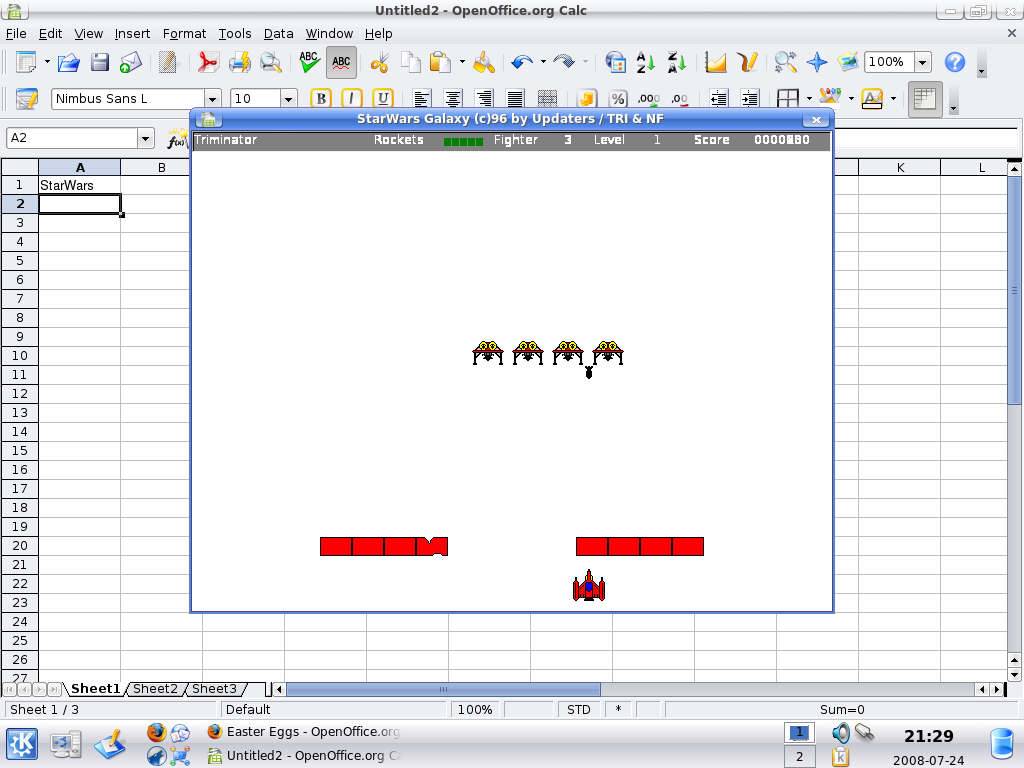
\includegraphics[width=0.70\textwidth]{images/chapter9/easteregg}
\caption[Easter Eggs]{Τα \emph{easter eggs} (αν δεν τα ξέρετε) είναι μικρά προγραμματάκια κρυμμένα μέσα σε μεγαλύτερα (και πολλές φορές ``σοβαρά προγράμματα'') τα οποία ενεργοποιούνται με κάποιο περίεργο, κρυφό τρόπο. Στις παλιές εκδόσεις του OpenOffice, υπήρχε κρυμμένο μέσα ένα παιχνίδι με τίτλο StarWars (μια ακόμα εκδοχή του Space Invaders στην πραγματικότητα). Για να ξεκινήσει έπρεπε κάποιος να γράψει {\tt =GAMES(“StarWars”)} στο πρώτο κελί. Δυστυχώς στις νέες εκδόσεις του openoffice και libreoffice τα easter eggs αφαιρέθηκαν.}
\label{9-1}
\end{figure}
%
\section{Η Αυτοκρατορία (των Χαζών) Αντεπιτίθεται!}
%
Ένα παιχνίδι που θα πυροβολάμε μόνο εξωγήινους χωρίς να μας αντεπιτίθενται θα γίνει βαρετό πολύ σύντομα: κάτι σαν το Graphics Match όπου μόνο χάναμε. Ήρθε η ώρα αυτά τα χαζά πλάσματα να αποκτήσουν λίγη αξιοπρέπεια προβάλλοντας μια κάποια αντίσταση.

Πριν ξεκινήσουμε, ας θυμηθούμε λίγο τις παραμέτρους στον constructor του {\tt Laser} class:

\begin{minted}[bgcolor=bg, frame=lines, framesep=10pt]{python}
class Laser:
  def __init__(self, coord, color, size, speed, refline, voffset):
\end{minted}

όπου φυσικά {\tt coord} είναι οι συντεταγμένες, {\tt color} είναι το χρώμα της βολής (διαφορετικό για τον εξωγήινο), {\tt size} είναι το μήκος της γραμμής Laser, {\tt refline} είναι η γραμμή αναφοράς εκκίνησης της βολής (το κάτω μέρος για τον εξωγήινο) και {\tt voffset} είναι μια μικρή διόρθωση στον κάθετο άξονα της βολής που μάλλον δεν θα χρειαστούμε για τα {\tt AlienShip}. Η συνάρτηση {\tt Fire} στο {\tt Alien} class θα είναι κάπως έτσι:

\begin{minted}[bgcolor=bg, frame=lines, framesep=10pt]{python}
def Fire(self):
  theshot = Laser((self.rect[0]+self.ship_midwidth,
                   self.rect[1]+self.firebaseline),self.firecolor,
                   self.shot_height, self.firespeed,
                   self.rect[1]+self.firebaseline, 0)
  return theshot
\end{minted}

Εννοείται ότι έχουμε ορίσει χρώμα, {\tt firebaseline} και {\tt shot\_height} στον constructor του {\tt Alien} class. 

Καλά όλα αυτά, αλλά δεν σημαίνει ότι οι εξωγήινοι ρίχνουν κιόλας. Θα πρέπει με κάποιο τρόπο να αποφασίζουν πότε (και αν) θα ρίξει ο καθένας τους. Δεν πρόκειται να βγάλουν χέρια και να χτυπάνε το {\tt SPACE} στο πληκτρολόγιο! (και αμφιβάλλουμε αν θα τους το δίνατε έτσι και αλλιώς). Για άλλη μια φορά θα μας σώσει η {\tt randint}:

\begin{minted}[bgcolor=bg, linenos, frame=lines, framesep=10pt]{python}
    for AlienShip in AlienShips:
      AlienShip.Show(screen)
      AlienShip.Move(time)
      if randint(0,10)==9:
        if alienfirelist:
          if alienfirelist[-1].DistanceTravelled()>=100:
            alienfirelist.append(AlienShip.Fire())
        else:
          alienfirelist.append(AlienShip.Fire())
\end{minted}

Ο εξωγήινος ρίχνει μόνο αν το {\tt randint(0,10)} φέρει την τιμή 9. Ναι, ουσιαστικά ο εξωγήινος\ldots{} ρίχνει ζάρι για να αποφασίσει αν θα ρίξει ή όχι. Και βέβαια μπορούμε να κάνουμε το παιχνίδι πιο δύσκολο γράφοντας κάτι σαν αυτό:
%
\begin{verbatim}
if randint(0,10)>4:
...
\end{verbatim}
%
οπότε και οι βολές θα είναι πιο συχνές. To {\tt alienfirelist} φυσικά είναι η λίστα που κρατάει τις εχθρικές βολές και αρχικοποιείται έξω από το βρόχο με την εντολή:

\begin{minted}[bgcolor=bg,  frame=lines, framesep=10pt]{python}
alienfirelist = []
\end{minted}

Ότι ισχύει για τις δικές μας βολές ισχύει και για τις εχθρικές: δεν ξεκινάει νέα βολή αν η προηγούμενη δεν έχει διανύσει μια ελάχιστη απόσταση που έχουμε ορίσει ως 100 pixels και ελέγχουμε με την {\tt DistanceTravelled()}. Δυστυχώς η {\tt DistanceTravelled()} όπως την έχουμε φτιάξει μέχρι στιγμής δεν λειτουργεί σωστά για τις εχθρικές βολές. Μπορείτε να φανταστείτε γιατί;

Απλά, οι βολές αυτές πηγαίνουν προς τα κάτω ενώ οι δικές μας προς τα πάνω. Έτσι, η συνάρτηση παράγει αρνητικές τιμές για τις εχθρικές βολές ενώ  στην ουσία μας ενδιαφέρει η απόλυτη τιμή αυτής της απόστασης. Και μόλις είπαμε την λέξη κλειδί για το πρόβλημα μας: η Python μας παρέχει την συνάρτηση απόλυτης τιμής {\tt abs} όπως σχεδόν όλες οι γλώσσες προγραμματισμού! Άρα η {\tt DistanceTravelled()} θα γίνει τώρα:

\begin{minted}[bgcolor=bg,  frame=lines, framesep=10pt]{python}
  def DistanceTravelled(self):
    return abs(self.refline – self.y1)
\end{minted}

Η αλλαγή αυτή δεν επηρεάζει φυσικά καθόλου τη λειτουργία της συνάρτησης στις δικές μας βολές.  Το μόνο που μένει είναι να δείξουμε και να κινήσουμε τις βολές:

\begin{minted}[bgcolor=bg,  linenos, frame=lines, framesep=10pt]{python}
  def DistanceTravelled(self):
    for theshot in alienfirelist:
      theshot.Move(time)
      theshot.Show(screen)
      if theshot.GoneBelow(laserdownlimit):
        alienfirelist.remove(theshot)
\end{minted}

Αντί για {\tt GoneAbove} έχουμε φυσικά {\tt GoneBelow} καθώς οι εχθρικές βολές κατευθύνονται προς τα κάτω (ή προς τα πάνω μας!). To {\tt laserdownlimit} το έχουμε ορίσει έξω από το βασικό βρόχο ως:

\begin{minted}[bgcolor=bg,  frame=lines, framesep=10pt]{python}
  laserdownlimit = screenheight – 40
\end{minted}

και φυσιολογικά θα έπρεπε να έχουμε και {\tt laseruplimit = 0} αντί να είναι hardcoded μέσα στον κώδικα (hint: φτιάξτε το!).  Είμαστε τώρα ένα βήμα πριν οι εξωγήινοι γίνουν επικίνδυνοι: ρίχνουν, αλλά είμαστε ακόμα άτρωτοι στις βολές τους.  Αυτό θα αλλάξει άμεσα!

\begin{SCfigure}
\centering
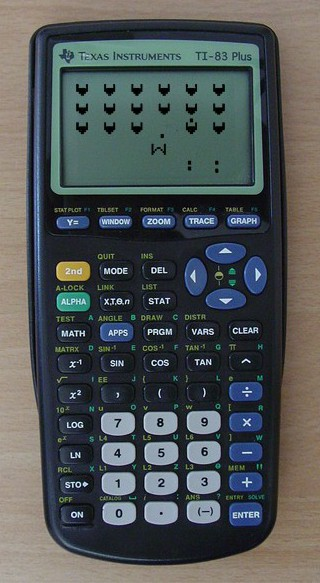
\includegraphics[height=0.95\textheight]{images/chapter9/calculator-invaders}
\caption[Calculator Invaders]{Τα παιχνίδια τύπου invaders είναι τόσο δημοφιλή που έχουν γραφτεί για τα πιο απίθανα μηχανήματα. Στη φώτο, space invaders για την προγραμματιζόμενη επιστημονική αριθμομηχανή (sic) ΤΙ-83 της Texas Instruments. Και τώρα ξέρετε τι δώρο να ζητήσετε από τους γονείς σας ως πρωτοετής φοιτητής. Για καθαρά εκπαιδευτικούς σκοπούς βέβαια!}
\label{9-2}
\end{SCfigure}

%
\section{Collision Detection Part II -- Οι Βολές Πέφτουν Βροχή!}
%
Εξασκηθείτε λίγο όσο οι εξωγήινοι είναι ακίνδυνοι: εδώ θα γράψουμε το collision detection για τις βολές που πέφτουν στο δικό μας σκάφος!  Είναι αρκετά όμοιο με το part I:

\begin{minted}[bgcolor=bg, linenos, frame=lines, framesep=10pt]{python}
    for theshot in alienfirelist:
      theshot.Move(time)
      theshot.Show(screen)
      if theshot.GoneBelow(laserdownlimit):
        alienfirelist.remove(theshot)
      else:
        if SpaceShip.rect.collidepoint(theshot.GetXY()):
          destroyed.play()
          if theshot in alienfirelist:
            alienfirelist.remove(theshot)
\end{minted}

Για κάθε εχθρική βολή που ταξιδεύει στην οθόνη μας:
%
\begin{itemize}
\item[-] Αν έχει βγει εκτός οθόνης εξαφανίζεται (αφαιρείται από τη λίστα {\tt alienfirelist})
\item[-] Διαφορετικά, αν έχει χτυπήσει το διαστημόπλοιο μας ακούγεται ο ήχος της έκρηξης (destroyed) και πάλι η βολή αφαιρείται από τη λίστα
\item[-] Αν δεν συμβαίνει τίποτα από τα δύο, η βολή απλώς συνεχίζει να κινείται.
\end{itemize}
%
Παρατηρήστε βέβαια ότι το διαστημόπλοιο μας δεν διαλύεται με τη βολή, όχι εμείς (θα) έχουμε ασπίδα! Χάνουμε όταν η ασπίδα μας πέφτει στο μηδέν. Όσο πετυχαίνουμε εξωγήινους η ασπίδα μας σιγά -- σιγά επανέρχεται. Μεγάλο πλεονέκτημα να είσαι προγραμματιστής τελικά: ορίζεις τους κανόνες του παιχνιδιού (προς το συμφέρον σου βέβαια!)

Για την ώρα δεν έχουμε όμως ούτε ασπίδα, ούτε καν score. Και έχουμε ένα ακόμα προβληματάκι: δεν υπάρχει καμιά ένδειξη στην οθόνη ότι έχουμε χτυπηθεί -- ακούγεται μόνο ένας ήχος. Όλα αυτά πρέπει φυσικά να τα φτιάξουμε.

\begin{figure}
\centering
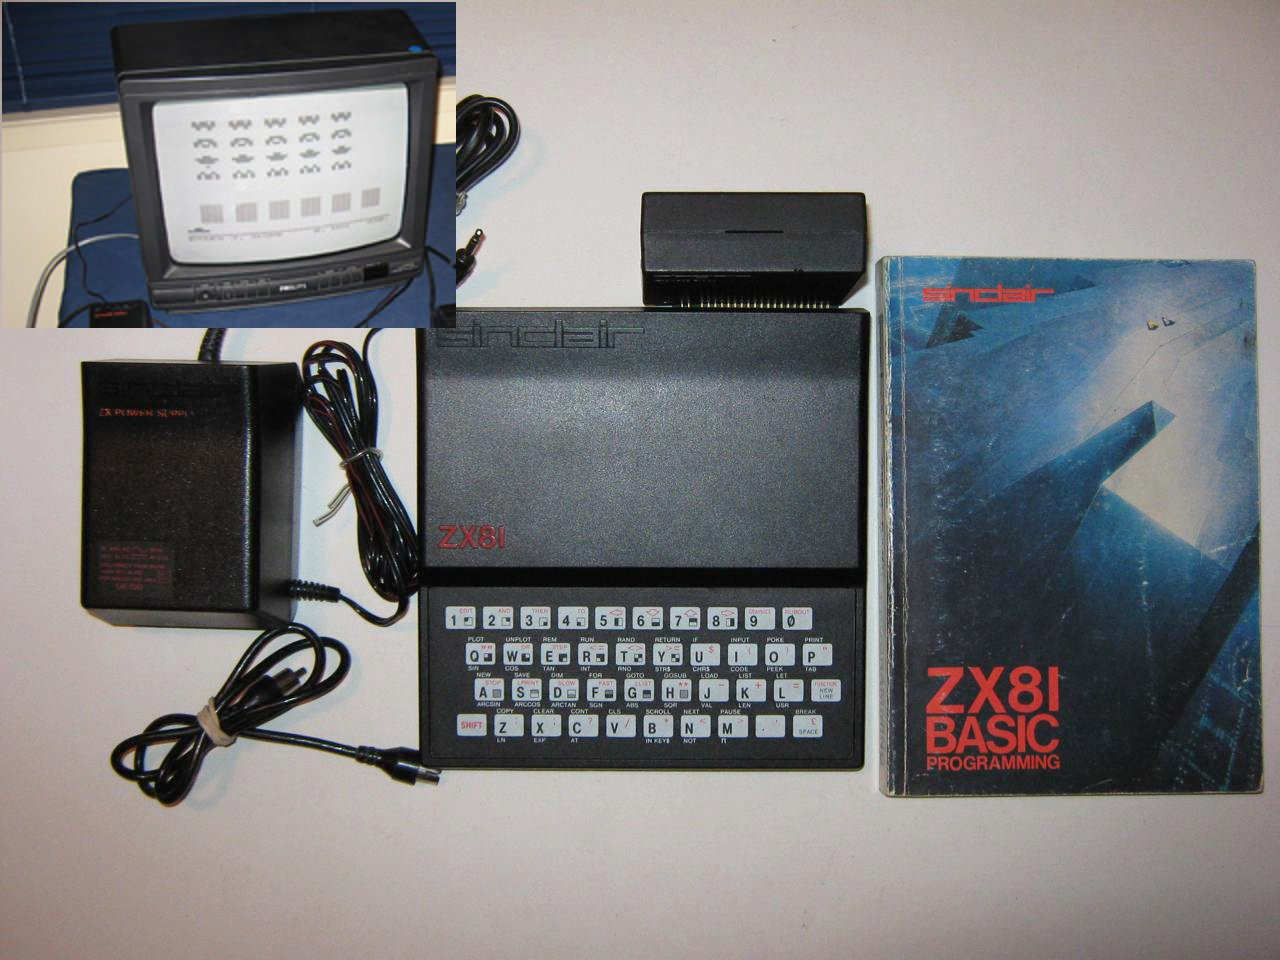
\includegraphics[width=0.80\textwidth]{images/chapter9/zx81-invaders}
\caption[ZX-81 Invaders]{O ZX-81, δημιούργημα της Sinclair Research, γνωστή από το ZX Spectrum, είναι ένα από τα πρώτα οικιακά micros με 1Kb RAM (και εξωτερική επέκταση στα 16Kb) με το καταπληκτικό χαρακτηριστικό ότι ήταν\ldots{} ασπρόμαυρο. Με ταχύτητα 1MHz ή 2MHz (το λεγόμενο\ldots{} fast mode) πάλι μπορούσε να τρέξει το Space Invaders όπως βλέπετε στη φώτο (προφανώς το συγκεκριμένο είναι γραμμένο σε assembly και όχι σε BASIC).}
\label{9-3}
\end{figure}
%
\section{Τήρηση Score}
%
Αυτό είναι εύκολο. Ορίστε μια πολύ απλή κλάση για το {\tt ScoreBoard}:

\begin{minted}[bgcolor=bg, linenos, frame=lines, framesep=10pt]{python}
class ScoreBoard:
  def __init__(self,x,y,font, fontsize):
    self.x = x
    self.y = y
    self.font = pygame.font.SysFont(font,fontsize)
    self.score = 0
        
  def Change(self, amount):
    self.score += amount

  def Show(self,surface):
    scoretext = self.font.render("Score: "+str(self.score), True, (0,0,255))
    surface.blit(scoretext,(self.x,self.y))

  def GetValue(self):
    return self.score

  def SetValue(self, score):
    self.score = score
\end{minted}

Είναι πιστεύουμε εντελώς προφανής: Το {\tt Score} θα εμφανίζεται στην θέση {\tt (x,y)} της οθόνης με τη γνωστή μας μέθοδο {\tt blit}. Έχουμε συναρτήσεις {\tt Change} για να προσθέσουμε στο score την τιμή {\tt amount} και {\tt GetValue / SetValue} για να διαβάσουμε την τιμή ή να θέσουμε το score απευθείας σε μια τιμή της αρεσκείας μας (πάλι στο cheat πάει το μυαλό σας ε;). Στο κύριο πρόγραμμα μας θα έχουμε:

\begin{figure}
\centering
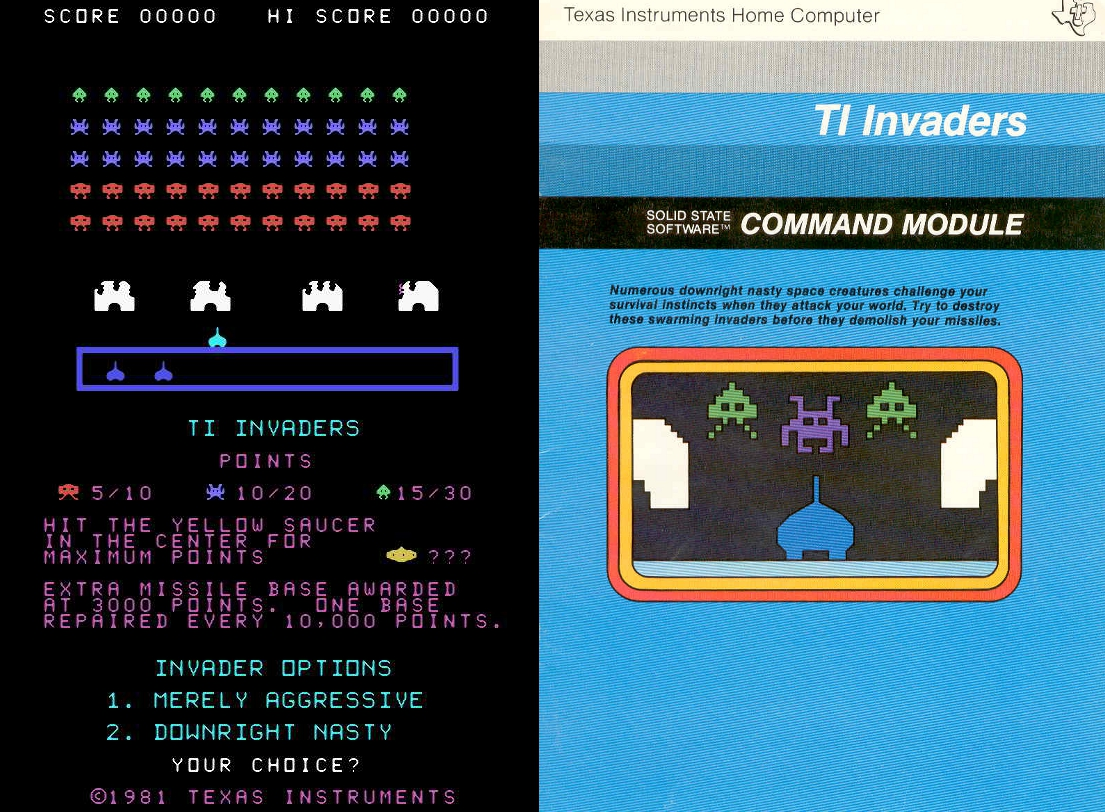
\includegraphics[width=0.70\textwidth]{images/chapter9/ti-invaders}
\caption[TI Invaders]{Στο προηγούμενο κεφάλαιο σας έδειξα την δική μου εκδοχή του TI Invaders, σε BASIC -- πριν καν μάθω ότι η TI είχε κυκλοφορήσει το Space Invaders σε cartridge.  Οι δύο φώτο είναι από το παιχνίδι, ενώ βλέπετε και τις οδηγίες του. Είναι αρκετά δύσκολο και γίνεται ακόμα χειρότερο αν προσπαθείτε να παίξετε με τα original TI joysticks (έχουν ψηφιστεί μέσα στα δέκα χειρότερα όλων των εποχών).}
\label{9-4}
\end{figure}

Αρχικοποίηση Score:

\begin{minted}[bgcolor=bg, frame=lines, framesep=10pt]{python}
  score = ScoreBoard(0,0,”impact”,32)
\end{minted}

Σε κάθε επιτυχία μας:

\begin{minted}[bgcolor=bg,  frame=lines, framesep=10pt]{python}
          if AlienShip.rect.collidepoint(theshot.GetXY()):
            score.Change(10)
\end{minted}

Για να δούμε όμως και αυτή την ασπίδα που λέγαμε, για να σταματήσουμε να παριστάνουμε τους\ldots{} Highlanders!

\begin{SCfigure}
\centering
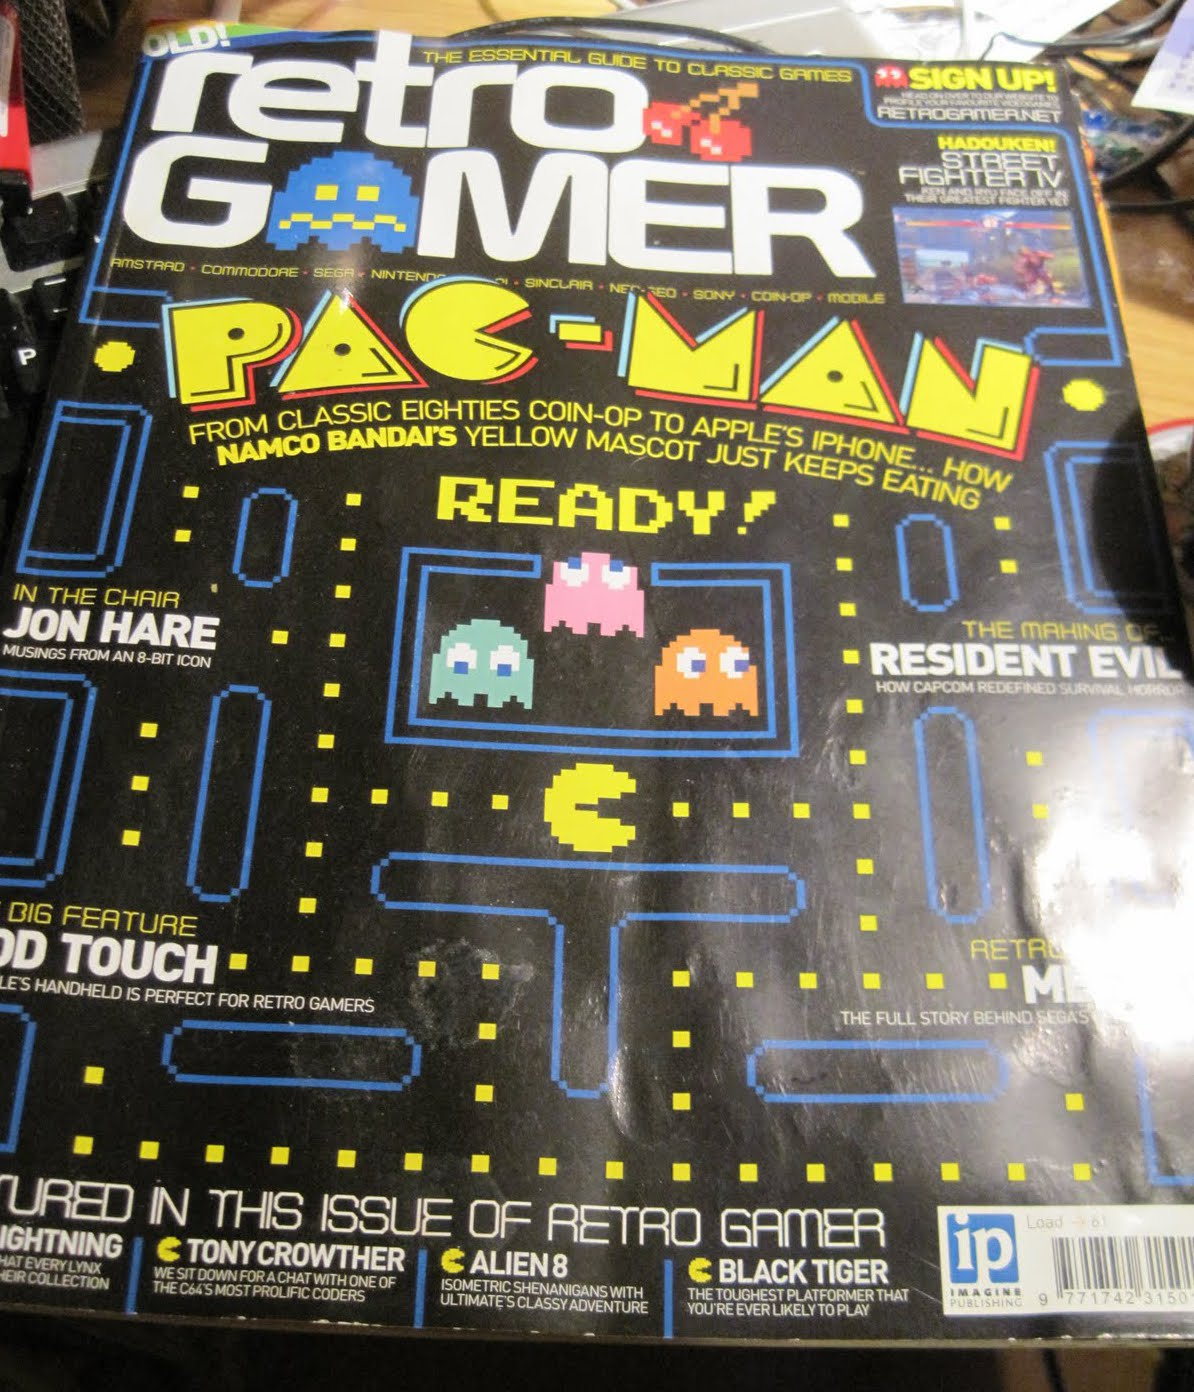
\includegraphics[width=0.60\textwidth]{images/chapter9/retro-pacman.jpg}
\caption[Pacman]{Όταν βαριόμασταν το Space Invaders σειρά είχε το Pacman. Άπειρα joysticks πρέπει να έχουν διαλυθεί εξαιτίας αυτών των δύο παιχνιδιών. Στη φώτο βλέπετε ένα από τα περιοδικά που ασχολείται με retro gaming -- και πρέπει να σας πληροφορήσω ότι η retro σκηνή καλά κρατεί. Οι περισσότεροι βέβαια χρησιμοποιούν πλέον εξομοιωτές, αλλά όσοι έχουν τα original μηχανήματα δεν τα αλλάζουν με τίποτα!}
\label{9-5}
\end{SCfigure}
%
\section{ShieldMeter Class: Μια Κλάση για την Ασπίδα μας!}
%
Το {\tt ShieldMeter} class είναι αρκετά απλό: σχεδιάζει μια μπάρα στην οθόνη που μειώνεται καθώς πέφτει η ενέργεια της ασπίδας μας (όσο δηλ. καθόμαστε και τις τρώμε άγρια από τους εξωγήινους) ή αυξάνεται μετά από κάποιες δικές μας πετυχημένες βολές. Αν η ασπίδα μας πέσει κάτω από κάποια τιμή ({\tt warnvalue}) το χρώμα της μπάρας αλλάζει. Προφανώς η ασπίδα έχει μια μέγιστη τιμή ({\tt maxvalue}) πέρα από την οποία δεν αυξάνεται και εννοείται δεν μπορεί να πάει κάτω από το μηδέν (στο μηδέν βλέπουμε ήδη τα ψηφιακά ραπανάκια να φυτρώνουν από κάτω). 

\begin{minted}[bgcolor=bg, frame=lines, framesep=10pt]{python}
class ShieldMeter:
  def __init__(self, x, y, maxvalue, warnvalue):
\end{minted}
 
Το μόνο ενδιαφέρον πρακτικά κομμάτι στον κώδικα είναι η σχεδίαση με την {\tt draw.rect}, οι άλλες συναρτήσεις είναι τόσο απλές όσο και του {\tt ScoreBoard}:

\begin{minted}[bgcolor=bg, linenos, frame=lines, framesep=10pt]{python}
  def Show(self, surface):
    if self.currentvalue < self.warnvalue:
      self.shieldcolor = (255,0,0)
    else:
      self.shieldcolor = (0,255,0)
    pygame.draw.rect(surface,self.shieldcolor,(self.x, self.y,  self.currentvalue,25))
\end{minted}

Το ``μαγικό'' 25 είναι το ύψος της μπάρας στην οθόνη. Μάλλον θα θέλετε να κάνετε κάτι για αυτό στον constructor, έτσι δεν είναι;

Στο κύριο πρόγραμμα, το {\tt shield} αρχικοποιείται ως εξής:

\begin{minted}[bgcolor=bg, frame=lines, framesep=10pt]{python}
  shield = ShieldMeter(200,10,250,75)
\end{minted}

όπου το 200,10 είναι οι συντεταγμένες εμφάνισης, το 250 είναι η μέγιστη τιμή και το 75 η τιμή προειδοποίησης. Σε κάθε\ldots{} τυχερή βολή των χαζοεξωγήινων χάνουμε 25 μονάδες ασπίδας:

\begin{minted}[bgcolor=bg, linenos, frame=lines, framesep=10pt]{python}
       if SpaceShip.rect.collidepoint(theshot.GetXY()):
         destroyed.play()
         shield.Decrease(25)
\end{minted}

ενώ κάθε φορά που το score μας διαιρείται ακριβώς με το 100, παίρνουμε 25 μονάδες ασπίδας:

\begin{minted}[bgcolor=bg, linenos, frame=lines, framesep=10pt]{python}
          if AlienShip.rect.collidepoint(theshot.GetXY()):
            score.Change(10)
            explosion.play()
            if score.GetValue() % 100 == 0:
              shield.Increase(25)
\end{minted}
 
Φυσικά μέσα στον κύριο βρόχο υπάρχει η εντολή {\tt shield.Show(screen)} για να εμφανίζεται η ασπίδα μας στην οθόνη!

\begin{SCfigure}
\centering
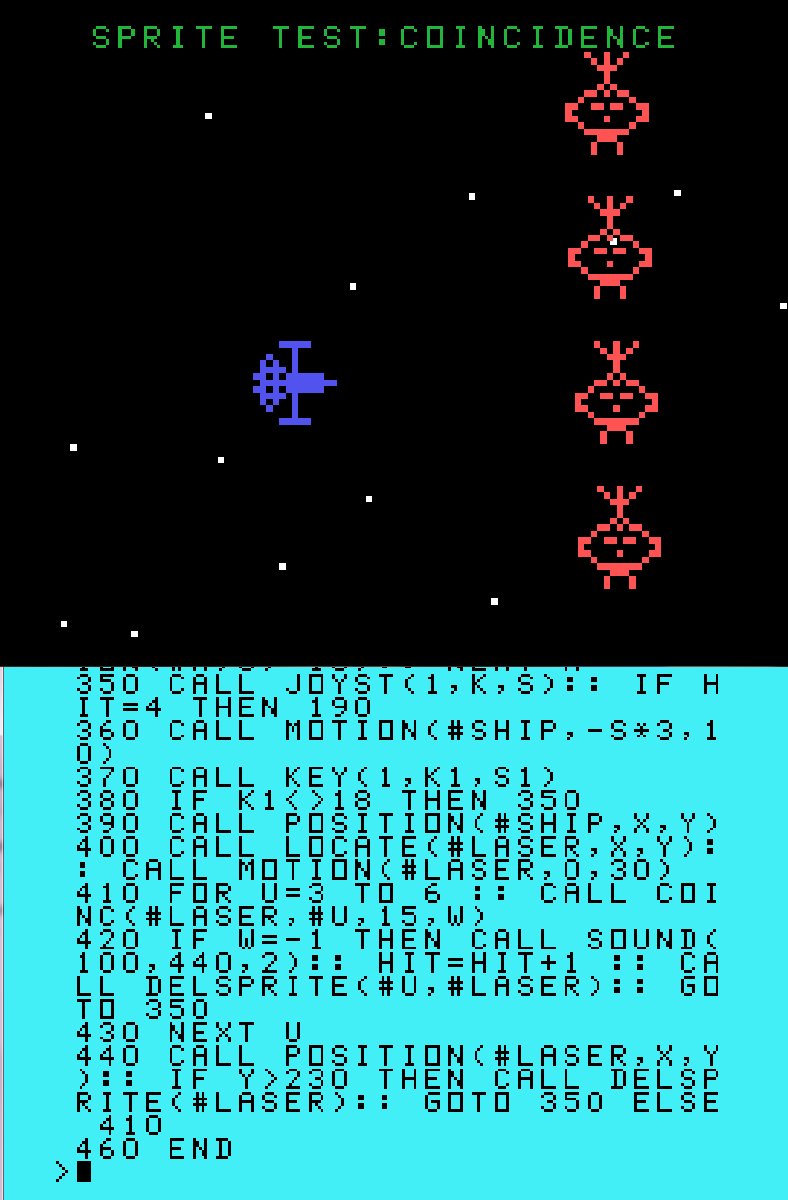
\includegraphics[width=0.50\textwidth]{images/chapter9/coincidence3}
\caption[Ανίχνευση Συγκρούσεων, the old way!]{Ανίχνευση συγκρούσεων με τον παλιό καλό (;) τρόπο. Τα sprites κινούνται αυτόματα και η σύγκρουση δεν γίνεται αντιληπτή αν δεν συμπέσει με την  εκτέλεση της εντολής ανίχνευσης. Στην TI Extended BASIC, η εντολή αυτή είναι η CALL COINC (από το coincidence, σύμπτωση) που φαίνεται στο listing.  Δείτε και το παρακάτω διασκεδαστικό video που δείχνει το πρόγραμμα και συγκρίνει το τότε με το τώρα: \url{http://www.youtube.com/watch?v=6rK7_2zrauM}}
\label{9-6}
\end{SCfigure}
%
\section{Ανίχνευση Τέλους Παιχνιδιού}
%
Όλα τα πράγματα έχουν ένα τέλος και μοιραία κάποια στιγμή οι εξωγήινοι θα σας φάνε λάχανο! Το παιχνίδι προφανώς πρέπει να ανιχνεύει το τέλος της ασπίδας σας, να δείχνει μήνυμα Game Over και να μην επιτρέπει να συνεχίσετε. Για το μήνυμα έχουμε μια πολύ απλή συνάρτηση {\tt GameOverShow} που κάνει {\tt blit} τα αντίστοιχα μηνύματα:

\begin{minted}[bgcolor=bg, linenos, frame=lines, framesep=10pt]{python}
def GameOverShow(screen):
  font = pygame.font.SysFont("impact", 32)
  gameovertext = font.render("Game Over!",True,(255,255,255))
  text_x = CenterMessage(screen, gameovertext)
  screen.blit (gameovertext,(text_x,280))
  gameovertext = font.render("Press R to Restart", True, (255,255,255))
  text_x = CenterMessage(screen, gameovertext)
  screen.blit(gameovertext,(text_x,320))
  return
\end{minted}

Όπως βλέπετε έχουμε προσθέσει και την pygame εκδοχή της {\tt CenterMessage} για το κεντράρισμα του κειμένου. Στον κύριο βρόχο έχουμε:

\begin{minted}[bgcolor=bg, frame=lines, framesep=10pt]{python}
    if shield.GetValue() == 0:
      GameOverShow(screen)
      GameOver = True
\end{minted}

Για να εξασφαλίσουμε ότι το παιχνίδι δεν παίζει όσο το {\tt GameOver = True} αλλά και να επιτρέψουμε την επανεκκίνηση του με το πλήκτρο R, έχουμε αλλάξει κατάλληλα τις εντολές στην ανίχνευση του πληκτρολογίου:

\begin{minted}[bgcolor=bg, frame=lines, framesep=10pt]{python}
        if key[K_SPACE] and not GameOver:
\end{minted}

To διαστημόπλοιο μας ρίχνει μόνο αν δεν έχει επέλθει το {\tt GameOver}. Κινείται όμως αριστερά -- δεξιά (demo mode!). Οι εξωγήινοι μας ρίχνουν, αλλά οι βολές τους περνάνε από μέσα μας χωρίς να μας πειράξουν επειδή έχουμε αλλάξει την γραμμή:

\begin{minted}[bgcolor=bg, frame=lines, framesep=10pt]{python}
if SpaceShip.rect.collidepoint(theshot.GetXY()) and not GameOver:
\end{minted}

Τέλος, πιέζοντας το R, ο χρήστης έχει δυνατότητα να ξαναπαίξει. Το παιχνίδι είναι τόσο εθιστικό άλλωστε, που ήταν αδύνατον να παραλείψουμε αυτό το\ldots{} feature:

\begin{minted}[bgcolor=bg, linenos, frame=lines, framesep=10pt]{python}
        if key[K_r] and GameOver:
          GameOver = False
          shield.SetValue(250)
          score.SetValue(0)
\end{minted}

Φυσικά η μεταβλητή {\tt GameOver} αρχικοποιείται έξω από το βρόχο ως {\tt GameOver = False}.

Επιτέλους, μετά από όλα αυτά έχουμε ένα πλήρως λειτουργικό παιχνίδι το οποίο θα μας διασκεδάσει με τις ώρες, τόσο να το παίζουμε όσο και να το επεκτείνουμε! Γιατί φυσικά, ο σωστός προγραμματιστής διασκεδάζει περισσότερο γράφοντας το παιχνίδι, παρά παίζοντας το. Εξάλλου, όσο παίζουμε ανακαλύπτουμε δυνατότητες και λειτουργίες που θέλουμε να προσθέσουμε: ο κώδικας μας έρχεται σε κύματα (σαν τους εξωγήινους ένα πράγμα) και δεν τελειώνει ποτέ.

Σε λίγο θα δούμε πως θα κάνετε το διαστημοπλοιάκι μας να αλλάζει χρώμα όταν δέχεται βολές -- ακούγεται απλό, αλλά θα διαπιστώσετε ότι χρειάζεται να μάθετε και νέα κόλπα για να γίνει σωστά. Θα συζητήσουμε ακόμα άλλες βελτιώσεις που μπορείτε να κάνετε στον κώδικα αλλά και ιδέες για να επεκτείνετε το παιχνίδι, μια πρόκληση που αφήνω αποκλειστικά στα χέρια σας και στην\ldots{} καφεΐνη που θα καταναλώσετε.

Όπως σας αποδείξαμε ο προγραμματισμός όχι μόνο δεν είναι βαρετός, αλλά αντίθετα αποτελεί την πιο ενδιαφέρουσα και δημιουργική ασχολία σε ένα υπολογιστή. Ελπίζουμε τα επιχειρήματα μας να ήταν πειστικά -- μην πείτε όχι: θα σας κυνηγήσω με το Laser!
